\documentclass[conference]{IEEEtran}
\IEEEoverridecommandlockouts
% The preceding line is only needed to identify funding in the first footnote. If that is unneeded, please comment it out.
\usepackage{cite}
\usepackage{amsmath,amssymb,amsfonts}
\usepackage{graphicx}
\usepackage{textcomp}

\usepackage{algorithm}
\usepackage[noend]{algpseudocode}
\usepackage{subfigure}
\usepackage{multirow}
\usepackage[hidelinks]{hyperref}


\usepackage{bbold}

\renewcommand{\algorithmicrequire}{\textbf{Input:}}
\renewcommand{\algorithmicensure}{\textbf{Output:}}

\def\BibTeX{{\rm B\kern-.05em{\sc i\kern-.025em b}\kern-.08em
    T\kern-.1667em\lower.7ex\hbox{E}\kern-.125emX}}
    
\bibliographystyle{IEEEtran}
\usepackage[show]{chato-notes}

\newcommand{\E}[1]{\cdot10^{#1}}

\let\oldReturn\Return
\renewcommand{\Return}{\State\oldReturn}

\renewcommand{\citedash}{--} 
    
\begin{document}

\title{SNM: Stochastic Newton Method for Optimization of Discrete Choice Models}

\author{

\IEEEauthorblockN{Gael Lederrey}
\IEEEauthorblockA{\small \textit{Transport and Mobility Laboratory} \\
\textit{\'Ecole Polytechnique F\'ed\'erale de Lausanne}\\
Station 18, CH-1015 Lausanne \\
\texttt{gael.lederrey@epfl.ch}}
\and
\IEEEauthorblockN{Virginie Lurkin}
\IEEEauthorblockA{\small \textit{Transport and Mobility Laboratory} \\
\textit{\'Ecole Polytechnique F\'ed\'erale de Lausanne}\\
Station 18, CH-1015 Lausanne \\
\texttt{virginie.lurkin@epfl.ch}}
\and
\IEEEauthorblockN{Michel Bierlaire}
\IEEEauthorblockA{\small \textit{Transport and Mobility Laboratory} \\
\textit{\'Ecole Polytechnique F\'ed\'erale de Lausanne}\\
Station 18, CH-1015 Lausanne \\
\texttt{michel.bierlaire@epfl.ch}}
}

\maketitle

\begin{abstract}
Optimization algorithms are rarely mentioned in the discrete choice literature. One reason may be that classic Newton-Raphson methods have been rather successful in estimating discrete choice parameters on available data sets of limited size. However, thanks to recent advances in data collection, abundant data about choice situations become more and more available and state-of-the art algorithms can be very computationally burdensome on these massive datasets.  In this paper, inspired by the good practices from the machine learning field, we introduce a Stochastic Newton Method (SNM) for the estimation of discrete choice models parameters. Our preliminary results indicate that our method outperforms (stochastic) first-order and quasi-newton methods. 
%Discrete Choice Models' software often used standard optimization algorithms. However, with the advent of Big Data, these algorithms will soon become a drawback for training such models. The field of Machine Learning has seen the emergence of many powerful first-order methods. Yet, they do not make use of second-order methods often due to the difficulty of computing the Hessian when having a massive amount of features. Discrete Choice Models are often much smaller than Machine Learning models. Therefore, it is possible to use second-order methods for optimizing such models. 

%In this article, we present a Stochastic Newton Method (SNM) for training Multinomial Logit models. We benchmarked this algorithm against standard first-order methods and quasi-newton methods. Also, we highlight one problem when using stochastic methods and propose a future fix for SNM.
\end{abstract}

\begin{IEEEkeywords}
Discrete Choice Models, Optimization
\end{IEEEkeywords}

\section{Introduction}
\label{sec:intro}

Discrete choice models (DCM) have become an essential operational tool in modeling individual behavior. Many success stories have been reported in the scientific studies related to the transportation field. Estimating those models requires to solve an optimization problem and yet, optimization algorithms are rarely mentioned in the discrete choice literature. One reason may be that classic nonlinear programming algorithms (i.e., Newton-Raphson method) have been rather successful in estimating discrete choice parameters on available data sets of limited size. Thanks to recent advances in data collection, abundant data about choice situations become more and more available. While offering a grand potential for a better understanding of human choices, these new data sources also brings new challenges for the community. Indeed algorithms classically embedded in state-of-the art discrete choice software's (such as Biogeme~\cite{bierlaire_biogeme:_2003} or Larch~\cite{newman_larch:_2016}) can be very computationally burdensome on these massive datasets. \\

In contrast, extracting useful information from big data sets is at the core of Machine Learning (ML). Primarily interested in achieving high prediction accuracy, ML algorithms have proved to be successful on models involving a huge number of parameters. Thus, large-scale machine learning models often involves both large volumes of parameters and large data sets. As such, first-order stochastic methods are a natural choice for large-scale machine learning optimization.  Due to the high cost of computing the full-Hessian, the second-order methods have been much less explored. And yet, algorithms exploiting second-order information are able to provide faster convergence. \\

For the sake of interpretability, discrete choice models usually have a much more restricted set of parameters than models typically investigated in the ML community. We therefore argue that it is possible to use second-order information to estimate these models. In this paper, inspired by the good practices from the ML field, we introduce a Stochastic Newton Method (SNM) for the estimation of discrete choice models parameters. We investigate the convergence of our algorithm by benchmarking it against standard first-order methods and quasi-newton methods using a simple multinomial logit model on a small data set. We present preliminary results that indicate that our method outperforms (stochastic) first-order and quasi-newton methods. However, the algorithm developed in this paper only constitutes a first step toward our final goal that is the development of an optimization method specifically designed to estimate discrete choice model parameters on big data sets. Further modifications are currently investigated to achieve faster convergence and to be able to deal with large data sets. \\

The remainder of this paper is structured as follows. In section~\ref{sec:rel_work}, we present some related works about first and second-order optimization methods. In Section~\ref{sec:methodo}, we describe the discrete choice model we use; the Stochastic Newton Method algorithm that we propose to estimate its parameters, as well as the first-order methods and quasi-newton methods that we use as benchmark to evaluate our algorithm. Section~\ref{sec:res} shows the results and we present our concluding remarks and future works in section~\ref{sec:conclusion}. 


%In the ``optimization world'', there are three main categories of iterative algorithms: first-order methods, quasi-newton methods, and second-order methods. Of course, many other types of algorithms for optimizing objective function in a constrained or unconstrained environment. However, recently much work has been done on iterative optimization algorithms, see Section, thanks to the Machine Learning community. Indeed, with the advent of Machine Learning since the last twenty years, many researchers have been working on new ways to optimize models. Even if computers have become more powerful years after years, Machine Learning models have become more and more complex. We often see Deep learning models with more than a million features. Thus, optimization's research for Machine Learning focusses on first-order methods. Indeed, computing the Hessian is quite tedious with a massive number of features. \\

%Currently, most of the Discrete Choice models' packages, , make use of standard optimization algorithms. Within the era of Big Data, we want to use more and more data to get more accurate models. However, most of those standard algorithms will struggle with huge datasets. Therefore, the good practice coming from Machine Learning is to use stochastic algorithms. Stochastic first-order methods are known to be very efficient. However, they have some drawback such as the loss of information on the curvature of the function, contain in the Hessian. For odd objective function, this information is sometimes required. Therefore, thanks to the reasonable size of Discrete Choice models, we argue that it is possible to use Second-order stochastic methods for training Discrete Choice models and that it outperforms the standard first-order methods and quasi-newton methods. 

%In this article, we first present some related work. Then, we describe the multinomial logit model used in our experiments as well as a novel second-order stochastic algorithm: Stochastic Newton Method (SNM). Then, we show that usual first-order methods struggles on optimizing Multinomial Logit model. Finally, we show that SNM outperforms standards first-order methods and quasi-newton methods. We also give one small weakness of this algorithm with a way to fix it in the future.

\section{Related Work}
\label{sec:rel_work}

Optimization plays a key role in Machine Learning, especially for developing efficient and scalable algorithms suited for large datasets and complex models. In this respect, first-order methods have been extensively explored, leading to many variants of the popular Stochastic Gradient Descent (SGD) algorithm. A well-known issue of standard first-order methods is that they tend to struggle when the curvature of the objective function is not homogeneous~\cite{sutton_two_1986}. 

%As stated earlier, optimization algorithms play an important role in Machine Learning. Indeed, if we want to use complex models, we need to use powerful optimization methods. First-order methods have been studied a lot, and many variants of the standard Stochastic Gradient Descent (SGD) exists. It is well known that standard first-order methods tend to struggle when the curvature of the objective function is not homogeneous~\cite{sutton_two_1986}.

Therefore, Quian describes a method using momentum to help the gradient in these particular situations~\cite{qian_momentum_1999}. Other first-order methods adapt the step size to the parameters, such as Adagrad~\cite{duchi_adaptive_2011}. Then, there is an iterative process between researchers trying to improve previous algorithms. Ruder~\cite{ruder_overview_2016} gives a good overview of first-order methods, from SGD up to complex and recent first-order algorithms such as Nadam~\cite{dozat_incorporating_2016} or AMSGrad~\cite{reddi_convergence_2018}. \\

More recently, with the help of more powerful computers, researchers have been looking at quasi-newton methods. Indeed, such method may be beneficial when first-order methods are struggling due to the lack of information from the curvature. The idea behind quasi-newton methods is to use the gradient to approximate the Hessian iteratively. BFGS algorithm~\cite{fletcher_practical_1987} is a standard quasi-newton method. Stochastic BFGS algorithms such as RES-BFGS~\cite{mokhtari_res:_2014}, a regularized stochastic BFGS, are used nowadays. Many researchers are trying to make use of the structure of the problem to find alternative versions of a given algorithm to perform better on this specific problem. For example, Gower {\it et al.}~\cite{gower_accelerated_2018} have implemented an alternative version of BFGS for Matrix Inversion. Keskar {\it et al.}~\cite{keskar_adaqn:_2016} have implemented adaQN, an adaptative quasi-newton method specifically designed for training Recurrent Neural Networks. Some researchers, such as Ye and Zhang~\cite{ye_nestrovs_2017}, are inspired by the progress on first-order methods to improve second-order methods. We also see some algorithms making use of Conjugate Gradient and stochasticity to create better algorithms as done by Byrd {\it et al.}~\cite{byrd_use_2011}. In the end, the most advanced and recent methods make use of quasi-newton methods, see~\cite{kiros_training_2013,bordes_sgd-qn:_2009,bordes_erratum:_2010,agarwal_second-order_2016}. However, very little work on second-order method, making use of the analytical Hessian, can be found in the literature.

\vspace{-0.2cm}
\section{Methodology}
\label{sec:methodo}

In this section, we present the model used in this article, several optimization algorithms as well as the Stochastic Newton Method\footnote{The code is available on github: \href{https://github.com/glederrey/IEEE2018\_SNM}{https://github.com/glederrey/IEEE2018\_SNM}}.

\subsection{Model}
\label{sec:model}

We use the {\it Swissmetro} dataset~\cite{bierlaire_acceptance_2001} and build a multinomial logit model denoted by $\mathcal{M}$:
\begin{align}
\label{eq:model}
V_{\text{Car}} &= \text{ASC}_{\text{Car}} + \beta_{\text{TT,Car}} \text{TT}_{\text{Car}} + \beta_{\text{C,Car}} \text{C}_{\text{Car}} + \beta_{\text{Senior}}\mathbb{1}_{\text{Senior}} \nonumber \\
\begin{split}
V_{\text{SM}} &= \text{ASC}_{\text{SM}} + \beta_{\text{TT,SM}} \text{TT}_{\text{SM}} + \beta_{\text{C,SM}} \text{C}_{\text{SM}} \\
& \quad + \beta_{\text{HE}} \text{HE}_{\text{SM}} + \beta_{\text{Senior}}\mathbb{1}_{\text{Senior}}
\end{split} \\
V_{\text{Train}} &= \text{ASC}_{\text{Train}} + \beta_{\text{TT,Train}} \text{TT}_{\text{Train}} + \beta_{\text{C,Train}} \text{C}_{\text{Train}} + \beta_{\text{HE}} \text{HE}_{\text{Train}} \nonumber
\end{align}
where $\mathbb{1}_{\text{Senior}}$ is a boolean variable equal to one if the age of the respondent is over 65 years olds, 0 otherwise, $C$ denotes the cost, $TT$ the travel time, and $HE$ the headway for the train and Swissmetro. For this model, we removed all observations with unknown choice, unkown age and non-positive travel time. This gives a total of 9,036 observations.\\
 
We first estimate the model with Biogeme~\cite{bierlaire_biogeme:_2003} to obtain the optimal parameter values and verify that all parameters are significant. However, we do not use the usual log-likelihood. Instead, we are using a normalized log-likelihood which simply corresponds to the log-likelihood divided by the number of observations. Therefore, the final normalized log-likelihood is $-0.7908$ and the parameters are given in Table \ref{tab:res_biogeme}.\\

\begin{table}
\centering
\renewcommand\arraystretch{1.2}
\begin{tabular}{l|cccc}
\multicolumn{1}{l}{} & {\bf Value} & {\bf Std err} & {\bf t-test} & {\bf p-value} \\ \cline{2-5}
$\text{ASC}_{\text{Car}}$ & 0 & - & - & - \\
$\text{ASC}_{\text{SM}}$ & $7.86\E{-1}$ & $6.93\E{-2}$ & 11.35 & 0.00 \\
$\text{ASC}_{\text{Train}}$ & $9.83\E{-1}$ & $1.31\E{-1}$ & 7.48 & 0.00 \\
$\beta_{\text{TT,Car}}$ & $-1.05\E{-2}$ & $7.89\E{-4}$ & -8.32 & 0.00 \\
$\beta_{\text{TT,SM}}$ & $-1.44\E{-2}$ & $6.36\E{-4}$ & -21.29 & 0.00 \\
$\beta_{\text{TT,Train}}$ & $-1.80\E{-2}$ & $8.65\E{-4}$ & -20.78 & 0.00 \\
$\beta_{\text{C,Car}}$ & $-6.56\E{-3}$ & $7.89\E{-4}$ & -8.32 & 0.00 \\
$\beta_{\text{C,SM}}$ & $-8.00\E{-3}$ & $3.76\E{-4}$ & -21.29 & 0.00 \\
$\beta_{\text{C,Train}}$ & $-1.46\E{-2}$ & $9.65\E{-4}$ & -15.09 & 0.00 \\
$\beta_{\text{Senior}}$ & -1.06 & $1.16\E{-1}$ & -9.11 & 0.00 \\
$\beta_{\text{HE}}$ & $-6.88\E{-3}$ & $1.03\E{-3}$ & -6.69 & 0.00
\end{tabular}
\caption{\label{tab:res_biogeme} Parameters of the optimized model $\mathcal{M}$ by Biogeme.}
\vspace{-0.8cm}
\end{table}

We also provide a normalized model $\bar{\mathcal{M}}$ where the values of travel time, cost, and headway have been divided by 100. The parameters for this normalized model are the same as model $\mathcal{M}$ except that the values of parameters associated to the features normalized are multiplied by 100. The reason behind this normalization is to have parameters close to each other, {\it i.e.} in the same order of magnitude, as opposed to the values in Table \ref{tab:res_biogeme} where the parameter values are in four orders of magnitude. \\

\vspace{-0.3cm}
\subsection{Stochastic Newton Algorithm (SNM)}
\label{sec:snm}

In this article, we present an algorithm called Stochastic Newton Method. Within Neural Networks, the number of features $K$ can easily exceed one million. Thus, this is leading to huge Hessian since it will have $K^2$ elements. Discrete Choice Models, on the other hand, tend to have a reasonable number of features. Indeed, since the primary purpose of Discrete Choice Models is explaining the behavioral aspect of the samples, the models cannot contain too many parameters. Therefore, the primary limitation of Newton methods encountered in Neural Networks is not valid for Discrete Choice models. Yet, one problem remains: the exponential growth of data. Indeed, computing the Hessian on many data can be as tedious as computing it for many features. Thus the need for a Stochastic Newton Method (SNM).

The main point of this algorithm is to compute a stochastic Hessian. We show here that computing a stochastic Hessian is possible for a Logit Model. The generalization can be applied to any finite-sum function as such as the log-likelihood of a Logit Model. Let $N$ denote the number of samples, $\mathcal{C}$ denote the choice set and $\mathcal{C}_n$ denote the choice set available for observation $n$ and define
\[
y_{in} = 
\begin{cases}
1 & \text{if observation $n$ chose alternative $i$}, \\
0 & \text{otherwise}.
\end{cases}
\]
The likelihood function for a choice model is given by
\begin{equation}
\mathcal{L}^* = \prod_{n=1}^N \prod_{i\in\mathcal{C}_n} P_n(i)^{y_{in}}
\end{equation}
where $P_n(i)$ denotes the probability that observation $n$ choses alternative $i$. For a Logit model, we can define this probability as
\begin{equation}
\label{eq:proba}
P_n(i) = \frac{e^{V_{in}}}{\sum_{j\in\mathcal{C}_n e^{V_{jn}}}}
\end{equation}
where $V_{in}$ denotes the utility of alternative $i$ for observation $n$. If we take the logarithm of Equation (\ref{eq:proba}), we get the log-likelihood:
\begin{align}
\label{eq:log-likelihood}
\mathcal{L} &= \sum_{n=1}^N\sum_{i\in\mathcal{C}_n} y_{in}\left( V_{in} - \ln \sum_{j\in\mathcal{C}_n}e^{V_{jn}} \right) \nonumber \\
&= \sum_{n=1}^N \left( \sum_{i\in\mathcal{C}_n} y_{in}V_{in} - \ln \sum_{j\in\mathcal{C}_n}e^{V_{jn}} \right) 
\end{align}
The second equality is done using the fact that $\sum_{i\in\mathcal{C}_n} y_{in} = 1$. We then update the log-likehood of Equation (\ref{eq:log-likelihood}) to create a normalized log-likelihood.
\begin{equation}
\label{eq:norm_ll}
\bar{\mathcal{L}} = \frac{1}{N}\mathcal{L} = \frac{1}{N} \sum_{n=1}^N \left( \sum_{i\in\mathcal{C}_n} y_{in}V_{in} - \ln \sum_{j\in\mathcal{C}_n}e^{V_{jn}} \right)
\end{equation}
This is done such that the value of the log-likelihood stay in the same magnitude of order for any subset of observations $\mathcal{I}$. Indeed, if we denote $\mathcal{L}_{\mathcal{I}}$ as the log-likelihood computed on the observation from $\mathcal{I}$ and $\mathcal{N}$ the set of all observations, we see that
\begin{align}
\label{eq:comp_ll}
\begin{split}
\mathcal{L}_{\mathcal{I}} &=  \sum_{n\in \mathcal{I}} \left( \sum_{i\in\mathcal{C}_n} y_{in}V_{in} - \ln \sum_{j\in\mathcal{C}_n}e^{V_{jn}} \right)  \\
&< \sum_{n\in \mathcal{I}} \left( \sum_{i\in\mathcal{C}_n} y_{in}V_{in} - \ln \sum_{j\in\mathcal{C}_n}e^{V_{jn}} \right) \\ &\quad + \sum_{n \in \mathcal{N} \smallsetminus \mathcal{I}} \left( \sum_{i\in\mathcal{C}_n} y_{in}V_{in} - \ln \sum_{j\in\mathcal{C}_n}e^{V_{jn}} \right) \\
&= \mathcal{L}
\end{split}
\end{align}
As shown in Equation (\ref{eq:comp_ll}), the standard log-likelihood cannot be compared on different set of data if they do not have the same number of data. Therefore, it can be shown that normalizing this log-likelihood as done in Equation (\ref{eq:norm_ll}) produces log-likelihood of same order of magnitude independently of the number of observations.\\

The first derivatives of $\bar{\mathcal{L}}$ with respect to the coefficient for $k=1,\ldots,K$ are given by
\begin{align}
\frac{\partial \bar{\mathcal{L}}}{\partial \beta_k} &= \frac{1}{N} \sum_{n=1}^N \left(\sum_{i\in\mathcal{C}_n} y_{in}\frac{\partial V_{in}}{\partial \beta_k} - \sum_{i\in\mathcal{C}_n}1 P_n(i) \frac{\partial V_{in}}{\partial \beta_k}\right) \nonumber \\
&= \frac{1}{N}\sum_{n=1}^N \sum_{i\in\mathcal{C}_n} \left(y_{in} - P_n(i)\right) \frac{\partial V_{in}}{\partial \beta_k} 
\end{align}
The second derivatives for $k=1,\ldots,K$ and $l=1,\ldots,K$ are given by
\begin{equation}
\label{eq:second_deriv}
\frac{\partial^2 \bar{L}}{\partial \beta_k \partial \beta_l} = - \frac{1}{N}\sum_{n=1}^N \sum_{i\in\mathcal{C}_n} P_n(i) W_{ink} W_{inl}
\end{equation}
where 
\[
W_{ink} = \left(\frac{\partial V_{in}}{\partial \beta_k} - \sum_{j\in\mathcal{C}_n} \frac{\partial V_{jn}}{\partial \beta_k}P_n(j)\right)
\]

From the definition of the second derivatives in Equation (\ref{eq:second_deriv}), it is easy to compute the second derivative for only one observation $o$.
\begin{equation}
\label{eq:second_deriv_1}
\left.\frac{\partial^2 \bar{L}}{\partial \beta_k \partial \beta_l}\right|_{m} = - \sum_{i\in\mathcal{C}_o} P_o(i) W_{iok} W_{iol}
\end{equation}

\begin{algorithm*}[t]
\caption{Stochastic Newton Method (SNM)}\label{algo:snm}
\begin{algorithmic}[1]
\Require{Starting parameter value ($\theta_0$), data ($\mathcal{D}$), function ($f$), gradient ($\nabla f$), Hessian ($\nabla^2 f$), number of epochs ($n_{ep}$), batch size ($n_{batch}$)}
\Ensure{Epochs ($e$), parameters ($\theta$), function values ($f_v$)}
\Function{SNM}{}
\State $(n_{\mathcal{D}}, m) = |\mathcal{D}|$ \Comment{Number of samples and parameters}
\State $n_{iter} \gets \lceil n_{ep}n_{\mathcal{D}}/n_{batch} \rceil$ \Comment{Number of iterations}
\State Initialize $e$, $\theta$ and $f_v$. Set $\theta[0] \gets \theta_{0}$
\For {$i = 0 \ldots n_{iter}$}
\State $e[i] \gets i\cdot n_{batch} /n_{\mathcal{D}}$ \Comment{Store the epoch}
\State $f_{v}[i] \gets f(\theta[i])$ \Comment{Store the function value}
\State \texttt{idx} $\gets n_{batch} $ values from $\mathcal{U}(0, n_{\mathcal{D}})$ without replacement
\State \texttt{grad} $\gets \nabla f_{\texttt{idx}}(\theta[i])$ \Comment{Gradient on the samples from \texttt{idx}}
\State \texttt{hess} $\gets \nabla^2 f_{\texttt{idx}}(\theta[i])$ \Comment{Hessian on the samples from \texttt{idx}}
\If {\texttt{hess} is non singular}
\State \texttt{inv\_hess} $\gets \texttt{hess}^{-1}$
\State \texttt{step} $\gets -\texttt{grad} \cdot \texttt{inv\_hess}$
\Else 
\State \texttt{step} $\gets \texttt{grad}$
\EndIf
\State $\alpha \gets $ Backtracking Line Search with \texttt{step} on the subset of data  with indices from \texttt{idx}
\State $\theta[i+1] \gets \theta[i] + \alpha \cdot \texttt{step}$
\EndFor
\State $e[n_{iter}] \gets n_{iter}\cdot n_{batch} /n_{\mathcal{D}}$
\State $f_{v}[n_{iter}] \gets f(\theta[n_{iter}])$

\Return $e$, $\theta$ and $f_v$
\EndFunction
\end{algorithmic}
\end{algorithm*}

From the definitions in Equations (\ref{eq:second_deriv}) and (\ref{eq:second_deriv_1}), we can conclude that the Hessian on a subset of the observations $\mathcal{I}$ is simply the average of the Hessians for each of observation $i\in\mathcal{I}$. \\

We present now the Stochastic Newton Method (SNM), see Algorithm~\ref{algo:snm}. The computation of both the stochastic gradient and the stochastic Hessian are done on lines 9 and 10. One particular feature of this algorithm is the computation of the direction for the next step. Indeed, with small batches, the Hessian may be singular. For example, it is possible that a variable associated with a parameter $\beta_k$ is always equal to 0 for a small batch, {\it e.g.} binary variables. Therefore, the derivative of $V_{in}$ by $\beta_k$ will always be zero. Therefore, the row and column of the Hessian will both be zero for this particular parameter, thus making it singular. The countermeasure to this possibility is to test if the Hessian is singular or not. If it is not the case, then the algorithm performs a standard Newton step with the stochastic Hessian and gradient. However, if the Hessian is singular, the algorithm performs a Stochastic Gradient Descent (SGD) step. Concerning the choice of the step size, for a given objective function, it often differs between SGD and Newton Method. Therefore, we have two possibilities: the algorithm should use two different step sizes, or we can perform a line search, as explained at the end of Section \ref{sec:algorithms}. 

\subsection{Benchmark algorithms}
\label{sec:algorithms}

We use several algorithms to train models $\mathcal{M}$ and $\bar{\mathcal{M}}$. These algorithms fall into three different categories: first-order methods, second-order methods, and quasi-newton methods. For first-order methods, we use mini-batch SGD~\cite{ruder_overview_2016} and Adagrad~\cite{duchi_adaptive_2011}. For the quasi-newton methods, we use BFGS algorithm~\cite{fletcher_practical_1987} and RES-BFGS~\cite{mokhtari_res:_2014}, a regularized stochastic version of BFGS. The main second-order algorithm is the Newton method~\cite{caswell_treatise_1685}. We run all the algorithms presented above with a backtracking Line Search method using the Armijo-Goldstein condition~\cite{armijo_minimization_1966} to avoid the long and tedious search of a good step size.


\section{Results}
\label{sec:res}

In this section, we show why first-order moethods tend to struggle to optimize Multinomial Logit Model. Then, we do a benchmark on multiple algorithms. Finally, we present a weakness of SNM and a future way to fix it.

\subsection{Raw data vs Normalized data}
\label{sec:norm_unorm}

Most of the data we can obtain are not normalized. This is often a preprocessing step required for some optimization algorithm to work. As explained in Section \ref{sec:model}, the optimization of the model leads to optimized parameters ranging over four orders of magnitude. Since the step size is the same for all parameters, it is difficult to find an optimal step size. Figure \ref{fig:sgd_norm_unorm} and \ref{fig:adagrad_norm_unorm} show the optimization process of the log-likelihood for SGD and Adagrad, respectively, for both the raw model $\mathcal{M}$ and the normalized model $\bar{\mathcal{M}}$. For both algorithms, the optimization was done ten times for ten epochs with a batch size of 100 observations. The lines correspond to the average while the colored part corresponds to the 95\% confidence interval. The results show that these algorithms perform better on the normalized model $\bar{\mathcal{M}}$. Table \ref{tab:res_norm_unorm} show the average value of the log-likelihood after two epochs for these two algorithms on both models.

\begin{figure*}[t]
    \centering
    \subfigure[SGD]{
        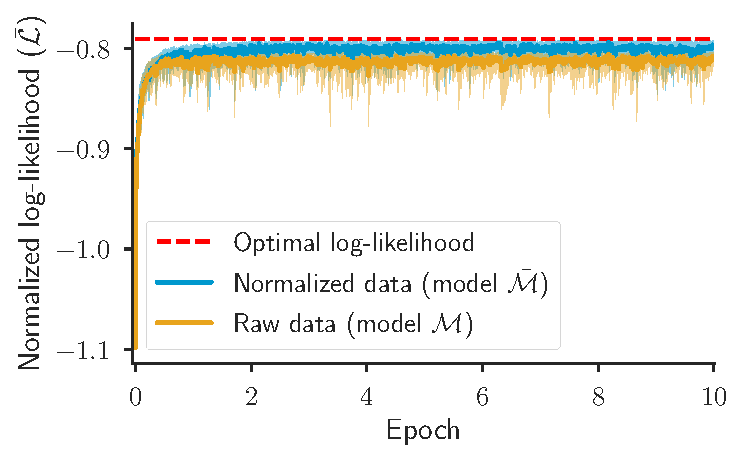
\includegraphics[width=0.3\textwidth]{../figures/SGD_norm_raw10.pdf}
        \label{fig:sgd_norm_unorm}
    }~
    \subfigure[Adagrad]{
        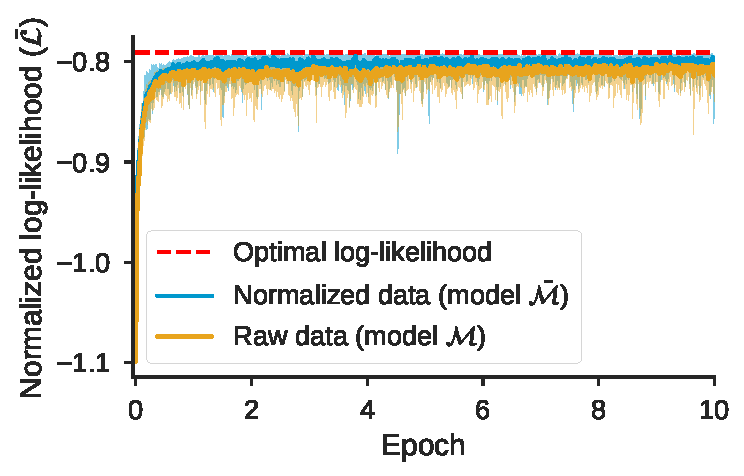
\includegraphics[width=0.3\textwidth]{../figures/adagrad_norm_raw10.pdf}
        \label{fig:adagrad_norm_unorm}
    }~
    \subfigure[SNM]{
        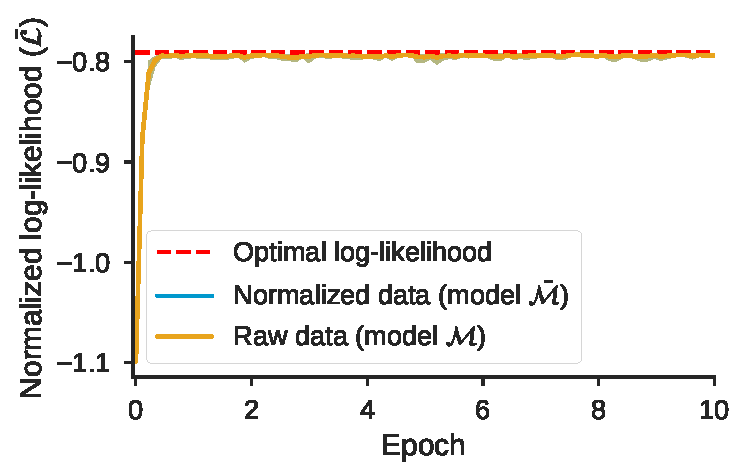
\includegraphics[width=0.3\textwidth]{../figures/SNM_norm_raw10.pdf}
        \label{fig:snm_norm_unorm}
    }
    \caption{Evaluation of the algorithms on raw data (model $\mathcal{M}$) and normalized data (model $\bar{\mathcal{M}}$). The vertical axis corresponds to the normalized log-likelihood presented in Equation (\ref{eq:norm_ll}). Each time, ten runs have been executed. The lines correspond to the average value over all the runs and the colored part correspond to the 95\% confidence interval. SGD and Adagrad are run with a batch size of 100 observations, SNM is run with a batch size of 1,000 observations.}
    \label{fig:norm_unorm}
    \vspace{-0.5cm}
\end{figure*}

\begin{table}
\centering
\renewcommand\arraystretch{1.2}
\begin{tabular}{l|ccc}
\multicolumn{1}{l}{} & {\bf SGD} & {\bf Adagrad} & {\bf SNM} \\ \cline{2-4}
on $\mathcal{M}$ & -0.813107 & -0.812080 & -0.794219 \\
on $\bar{\mathcal{M}}$ & -0.801739 & -0.801646
 & -0.794219 \\ \hline
rel. diff.  & 1.42\% & 1.30\% & 0.00\%
\end{tabular}
\caption{\label{tab:res_norm_unorm} Average normalized log-likelihood over a thousand runs at the second epoch for SGD, Adagrad and SNM.}
\vspace{-0.9cm}
\end{table}

Figure \ref{fig:snm_norm_unorm} shows the results of the training on both models with SNM. We ran this algorithm with batches of 1,000 observations. In Sections \ref{sec:comp_algo} and \ref{sec:effect_bs}, we explain why we had to use a batch size with more observations. The qualitative results as well as the quantitative results in Table \ref{tab:res_norm_unorm} show that second-order methods have less problem with badly conditioned optimization problem. Thus, it indicates that the information contained in the Hessian is important when the problem is ill-conditioned.

\subsection{Comparison of the algorithms}
\label{sec:comp_algo}

In this section, we want to compare the three main categories of algorithms: first-order methods, quasi-newton methods, and second-order methods. Figure \ref{fig:first_order} shows the results for SGD with batch size of 100 and 1,000 as well as gradient descent. Figure \ref{fig:quasi_newton} shows the results for RES-BFGS with batch sizes of 100 and 1,000 as well as standard BFGS. Finally,  Figure Figure \ref{fig:second_order} shows the results for SNM with batch sizes of 100 and 1,000 as well as Newton method. For these three figures, we executed ten runs. The lines give the average value for the normalized log-likelihood, and the colored parts show the 95\% confidence interval.\\

\begin{figure*}[t]
    \centering
    \subfigure[First-order methods]{
        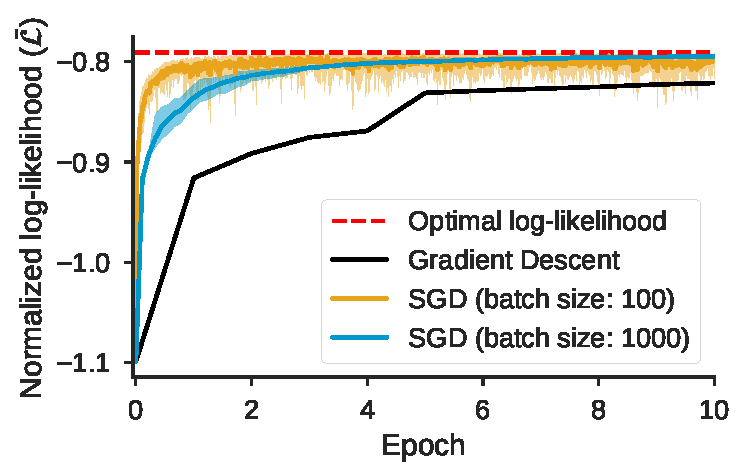
\includegraphics[width=0.3\textwidth]{../figures/SGD10.pdf}
        \label{fig:first_order}
    }~
    \subfigure[Quasi-Newton methods]{
        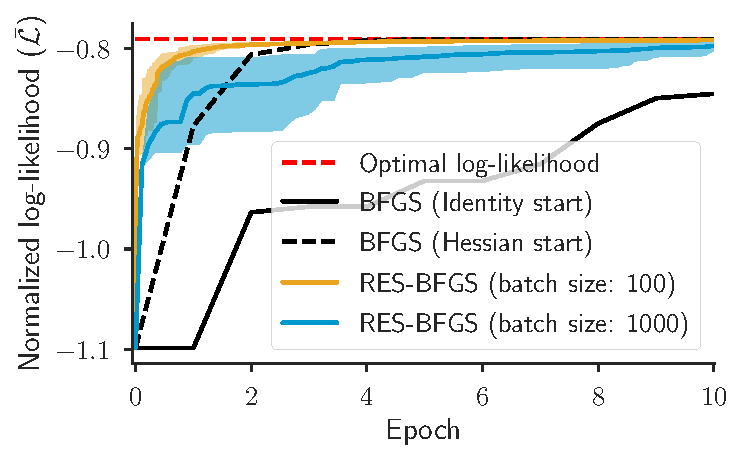
\includegraphics[width=0.3\textwidth]{../figures/SBFGS10.pdf}
        \label{fig:quasi_newton}
    }~
    \subfigure[Second-order methods]{
        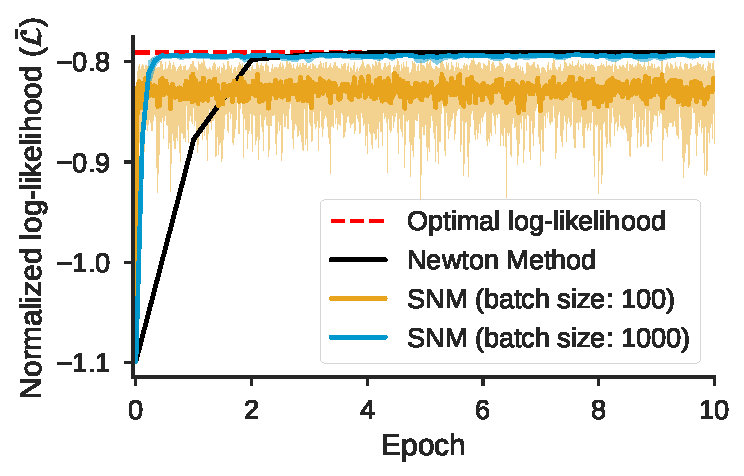
\includegraphics[width=0.3\textwidth]{../figures/SNM10.pdf}
        \label{fig:second_order}
    }
    \caption{Comparison of the different algorithms presented in Section \ref{sec:algorithms} and \ref{sec:snm}. The vertical axis corresponds to the normalized log-likelihood presented in Equation (\ref{eq:norm_ll}). Each time, a ten runs have been executed. The lines correspond to the average value over all the runs and the colored part correspond to the 95\% confidence interval.}
    \label{fig:comparison_algo}
    \vspace{-0.5cm}
\end{figure*}

\begin{table}
\centering
\renewcommand\arraystretch{1.2}
\begin{tabular}{lc|ccc}
&\multicolumn{1}{c}{batch} & {\bf first-order} & {\bf quasi-newton} & {\bf second-order} \\ \cline{3-5}
\multirow{ 2}{*}{\bf Stochastic} & 100 & -0.801452 & -0.796492 & -0.828409 \\
& 1000 & -0.812886 & -0.837937 & -0.794219 \\
\multicolumn{2}{l|}{\bf Full batch size}  & -0.891737 & -0.963458/-0.806245 & -0.798112
\end{tabular}
\caption{\label{tab:comparison_algo} Average normalized log-likelihood over a thousand runs at the second epoch for first-order methods, quasi-newton methods and second-order methods.}
\vspace{-0.8cm}
\end{table}

From Figure~\ref{fig:comparison_algo}, we already see that first-order methods are the furthest from the optimal value. Then, we see that stochastic quasi-newton methods tend to struggle to reach the optimal value, especially with the first approximation of the Hessian being an identity matrix. Interestingly, we see that the RES-BFGS works better with smaller batch size while it tends to struggle and plateau with big batch size. Nevertheless, it can get closer to the optimal solution than SGD. However, SNM is the best algorithm out of the three. Table \ref{tab:comparison_algo} gives the average value of the normalized log-likelihood for the second epoch. In this table, we reported two values for the quasi-newton method and the full batch size: the first value reported is with the first approximation of the Hessian being an identity matrix, the second value corresponds to the real hessian. The numbers confirm that SNM is the best algorithm. However, it is interesting to note that contrary to the other two algorithms, SNM runs better with bigger batch size. In the next section, see Section~\ref{sec:effect_bs}, we study the reason behind this behavior.

\subsection{Effect of the batch size}
\label{sec:effect_bs}

As shown in Figure~\ref{fig:comparison_algo}, SNM is the only algorithm for which a more significant batch size works better. This behavior is quite odd, and the explanation may come from the direction. Indeed, as explained in Section~\ref{sec:snm}, the direction is either a gradient step or a Newton step depending on the singularity of the Hessian. Therefore, we are interested to know if this direction, {\it i.e.} the choice between a gradient step and a Newton step, depends on the batch size. In Figure \ref{fig:perc_newton}, we show the percentage of Newton step that the algorithm is capable of performing in function of the batch size. This percentage is computed on a thousand draws. \\

\begin{figure}[t]
\centering
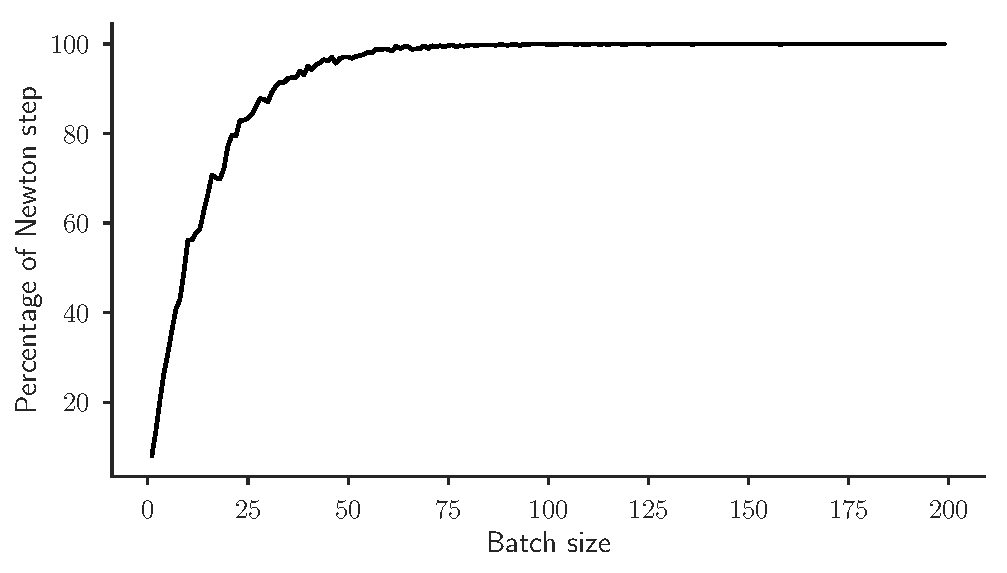
\includegraphics[width=0.45\textwidth]{../figures/perc_newton.pdf}
\vspace{-0.3cm}
\caption{Theoretical percentage of Newton step in function of the batch size for model $\bar{\mathcal{M}}$. The percentage was computed on a thousand draws.}
\label{fig:perc_newton}
\vspace{-0.3cm}
\end{figure}

The algorithm is only capable of performing a Newton step if the Hessian is non-singular. If we take a look at model $\mathcal{M}$, Equation~\ref{eq:model}, we see that we have one binary variable: $\mathbb{1}_{Senior}$. On our 9,036 observations, 8,406 observations have a 0 value for $\mathbb{1}_{Senior}$. In the particular case where all observations from a given batch have a 0 for $\mathbb{1}_{Senior}$, the hessian will be singular. However, as shown in Figure~\ref{fig:perc_newton}, this percentage goes quickly to 100\%. With a batch size of 100 observations, the algorithm will perform a Newton step 99.86\% of the time. Thus, we see that having binary variables that are often equal to 0 is not a problem for the algorithm. \\

However, small batch sizes create other problems. Indeed, when computing the Hessian with small batch size, the only information we get is from a small subset of the data. Therefore, for a given batch, the optimum can be different from the optimum on the whole dataset. Using the well optimized function \texttt{minimize} from the package \texttt{scipy.optimize}, we compute the optimum for different batch size. Then, we compare the euclidian distance between the optimum on the full dataset and the optimum from the different batches. Figure \ref{fig:batch_dist} shows the results of this experiment.

\begin{figure}[t]
\centering
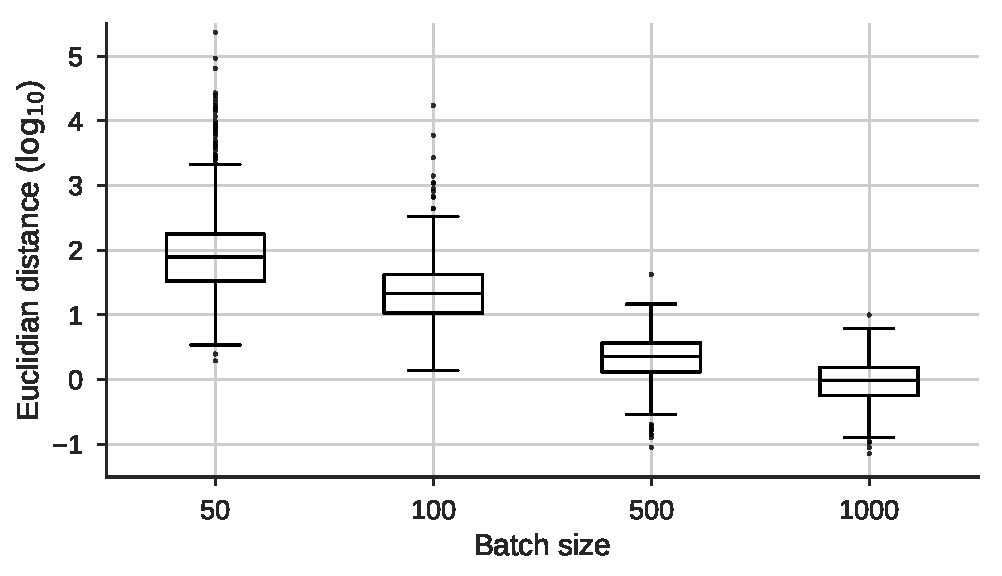
\includegraphics[width=0.45\textwidth]{../figures/dist.pdf}
\vspace{-0.3cm}
\caption{Euclidian distance between the optimal parameters obtained on the full dataset and optimal parameters found on batches of the data for different batch sizes. The line in the middle represents the median. A thousand draws were coomputed for each batch size.}
\label{fig:batch_dist}
\vspace{-0.5cm}
\end{figure}

In Figure~\ref{fig:batch_dist}, we see that when taking small batches, the optimal solution is pretty far from the optimal solution on all data point. Therefore, this creates a problem in the computation of the step for SNM. Indeed, since we do not take into account previous Hessian, as opposed to RES-BFGS, the algorithm will often change direction with small batches. Indeed, every time we change the batch, the algorithm is chasing a different optimum. Thus, it makes it difficult for it to achieve the real optimum. One way to fix this problem is to keep the information about previous Hessian and use this information to correct the direction of the algorithm.

\section{Conclusion}
\label{sec:conclusion}

In this article, we tested several algorithms to optimize a Multinomial Logit Model. We showed that first-order methods have many limitations on these particular models. In the comparison process, we added a stochastic quasi-newton method and introduced a new stochastic second-order method called SNM. To be able to use such an algorithm, we showed that computing the Hessian on only one observation (or a batch of observations) is legit thanks to the finite-sum shape of the log-likelihood. We then showed that this new method works particularly well to optimize our model. Also, we presented the main weakness of this method and the beginning of the solution to fix.. \\

Obviously, the next step is to fix the weakness of SNM. However, it is not a straightforward step. Indeed, we can merge the previous Hessian in may different ways and they will have to be tested. Nevertheless, with this new methodology in mind, many questions arise. As shown, we only tested our method on simple multinomial logit models. However, Discrete Choice theory contains many complex models such as Nested Logit Models, Cross-Nested Logit Models, and even models with Panel data. All of these models, on the contrary of Multinomial Logit Models, are not convex. Therefore, the optimization will be much more complicated. However, before experimenting with more complex models, it would be interesting to study the theoretical aspects of this model. Indeed, for the moment, we do not know the theoretical convergence rate of this algorithm. Thus, some theoretical work is required on this method. Finally, we also saw that making use of the model's structure can lead to good performance. For example, Latent variables require many draws from their probability distribution to be correctly estimated. Therefore, future algorithms should optimize while taking into account this structure. The same goes for models with Panel data. For this kind of models, the addition of a dimension is tricky when optimizing with standard methods. 

\section{Acknowledgements} 
\label{sec:acknowledgements}

We would like to thank Tim Hillel for his valuable insight on the development of this method as well as his comments that significantly improved this article.

\bibliography{PhD.bib}

\end{document}
